\documentclass[12pt,a4paper]{report}


\usepackage{amsmath}
\usepackage[utf8]{inputenc}
\usepackage{amsmath}
\usepackage{amsfonts}
\usepackage{amssymb}
\usepackage{calrsfs}
\usepackage[left=2cm,right=2cm,top=2cm,bottom=2cm]{geometry}
\usepackage[mathscr]{euscript}

%%%%%For writing large opertors%%%%%%%%%%%
%\usepackage{stmaryrd}
%%%%%%%%%%%%%%%%%%%%%%%%%%%%%%%%%%%%%%%%%%

%%%%%%%%%%for writing large parallel%%%%%%
\usepackage{mathtools}
\DeclarePairedDelimiter\bignorm{\lVert}{\rVert}
%%%%%%%%%%%%%%%%%%%%%%%%%%%%%%%%%%%%%%%%%%

%%%for drawing commutative diagrams.%%%%%%
\usepackage{tikz-cd}  
%%%%%%%%%%%%%%%%%%%%%%%%%%%%%%%%%%%%%%%%%%

%%%%%%%%%%for changing margin
\def\changemargin#1#2{\list{}{\rightmargin#2\leftmargin#1}\item[]}
\let\endchangemargin=\endlist 

\newenvironment{proof}
{\begin{changemargin}{1cm}{0.5cm} 
	}%your text here
	{\end{changemargin}
}

\newenvironment{subproof}
{\begin{changemargin}{0.5cm}{0.5cm} 
	}%your text here
	{\end{changemargin}
}
%%%%%%%%%%%%%%%%%%%%%%%%%%%%%

%%%%%%%%%%%%%%double rules%%%%%%%%%%%%%%%%%%%
\usepackage{lipsum}% Just for this example

\newcommand{\doublerule}[1][.4pt]{%
  \noindent
  \makebox[0pt][l]{\rule[.7ex]{\linewidth}{#1}}%
  \rule[.3ex]{\linewidth}{#1}}
%%%%%%%%%%%%%%%%%%%%%%%%%%%%%%%%%%%%%%%%%%%%%%

\begin{document}
\newcommand{\thm}{\textbf{Theorem) }}
\newcommand{\thmnum}[1]{\textbf{Theorem #1) }}
\newcommand{\defi}{\textbf{Definition) }}
\newcommand{\definum}[1]{\textbf{Definition #1) }}
\newcommand{\lem}{\textbf{Lemma) }}
\newcommand{\lemnum}[1]{\textbf{Lemma #1) }}
\newcommand{\prop}{\textbf{Proposition) }}
\newcommand{\propnum}[1]{\textbf{Proposition #1) }}
\newcommand{\corr}{\textbf{Corollary) }}
\newcommand{\corrnum}[1]{\textbf{Corollary #1) }}
\newcommand{\pf}{\textbf{proof) }}

\newcommand{\lap}{\triangle} %%Laplacian
\newcommand{\s}{\vspace{10pt}}
\newcommand{\bull}{$\bullet$}
\newcommand{\sta}{$\star$}
\newcommand{\reals}{\mathbb{R}}

\newcommand{\eop}{\hfill  \textsl{(End of proof)} $\square$} %end of proof
\newcommand{\eos}{\hfill  \textsl{(End of statement)} $\square$} %end of proof


\newcommand{\intN}{\mathbb{Z}_N}
\newcommand{\nat}{\mathbb{N}}
\newcommand{\norms}[2]{\bignorm[\big]{#1}_{#2}}
\newcommand{\abs}[1]{\big| #1 \big|}
\newcommand{\avg}{\mathbb{E}}
\newcommand{\prob}{\mathbb{P}}
\newcommand{\borel}{\mathscr{B}}
\newcommand{\EE}{\mathscr{E}}
\newcommand{\pa}{\partial}
\newcommand{\loc}{L^1_{\text{loc}}}

\renewcommand{\vec}{\underline}
\renewcommand{\bar}{\overline}

\def\doubleunderline#1{\underline{\underline{#1}}}

\newcommand{\newday}{\doublerule[0.5pt]}
\newcommand{\digression}{**********************************************************************************************}


\setlength\parindent{0pt}

\chapter*{Analysis of PDEs}
\s

\newday

(23rd November, Friday)
\s

\section*{Initial-Boundary Value Problems for Wave Equations}

Suppose $U\subset \reals^n$ is open with $C^1$-boundary. We define 
\begin{align*}
U_T = U \times (0,T), \quad \Sigma_t = U \times \{t \}, \quad \pa^* U_T = \pa U \times [0,T]
\end{align*}
\begin{figure}[h]
	\begin{center}
		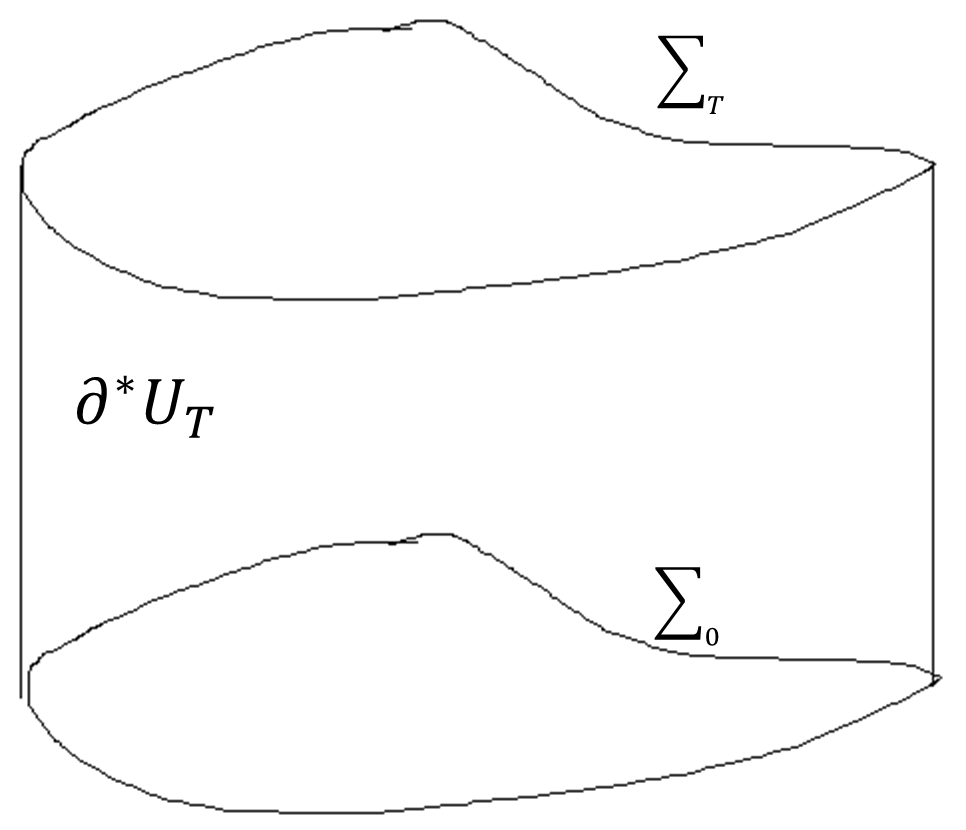
\includegraphics[scale=0.33]{9}
	\end{center}
\end{figure}
So $\pa U_T = \Sigma_0 \sqcup \Sigma_T \sqcup \pa^* U_T$. We define
\begin{align*}
Lu = -\sum_{i,j=1}^n (a^{ij}u_{x_i})_{x_j} + \sum_{i=1}^n b^i u_{x_i} + bu_t + cu
\end{align*}
where $a^{ij}, b^i, b,c \in C^1(\bar{U}_T)$. Further assume $a^{ij}$ satisfy the uniform ellipticity condition
\begin{align*}
\sum_{i,j=1}^n a^{ij}(x,t) \xi_i \xi_j \geq \theta |\xi|^2
\end{align*}
for some $\theta >0$, all $(x,t)\in U_T$, $\xi \in \reals^n$.

\quad The \textbf{initial-boundary value problem(IBVP)} we consider is:
\begin{align}
\begin{cases}
\begin{array}{ll}
u_{tt} + Lu = f & \text{in } U_T \\
u = \psi, \,\, u_t = \psi' & \text{on } \Sigma_0\\
u = 0 & \text{on } \pa^* U_T
\end{array}
\end{cases} \label{31}
\end{align}
e.g. The model in our mind is solving wave equation on a string given boundary conditions. If $L = - \Delta$, $f=0$, this is the wave equation on a bounded domain with specified initial conditions.
\s

As with the elliptic boundary value problem, we first find a weak formulation of the problem. Suppose $u\in C^2(\bar{U}_T)$ is a solution of (\ref{31}) and multiply the equation by $v\in C^2(\bar{U}_T)$ satisfying $v=0$ on $\pa^* U_T \cup \Sigma_T$. Then integrate over $U_T$.
\begin{align*}
\int_0^T dt \int_U dx (u_{tt} v + Luv) = \int_0^T dt \int_U dx fv
\end{align*}
Integrating by parts, we find
\begin{align}
\int_{U_T} \Big( -u_t v_t + \sum_{i,j} a^{ij}u_{x_i} v_{x_j} + \sum_i b^i u_{x_i} v + bu_t v  + cuv \Big) dxdt - \int_{\Sigma_0} \psi' v dx = \int_{U_T} fv dx dt \label{32}
\end{align}
Conversely, if (\ref{32}) holds for all $v\in C^2(\bar{U}_T)$ which vanish on $\Sigma_T \cup \pa^* U_T$ and $u\in C^2(\bar{U}_T)$ satisfies $u= \psi$ on $\Sigma_0$, $u=0$ on $\pa^* U_T$, undoing the integration by parts gives
\begin{align*}
\int_{U_T} (u_{tt}v + Lv - fv) dxdt + \int_{\Sigma_0} (u_t - \psi') vdx =0
\end{align*}
Taking $v\in C_c^{\infty}(U_T)$, the $\Sigma_0$ term vanishes and we deduce $u_{tt} + Lu = f$ in $U_T$. This implies
\begin{align*}
\int_{\Sigma_0} (u_t - \psi') vdx =0 \quad \forall v \in C_c^{\infty}(\Sigma_0) \quad \Rightarrow \quad u_t = \psi'
\end{align*}
The expression (\ref{32}) makes sense if $u\in H^1(U_T)$, $v\in H^1(U_T)$. This motivates the definition :
\s

\defi Suppose $f\in L^2(U_T)$, $\psi \in H_0^1(\Sigma_0)$, $\psi \in L^2(\Sigma_0)$ and $a^{ij}, b^i, b, c \in C^1(\bar{U}_T)$ with $a^{ij}$ satisfying uniform ellipticity condition in $U_T$. We say $u\in H^1(U_T)$ is a weak solution of the IBVP (\ref{31}) if
\begin{align*}
\begin{cases}
\begin{array}{lll}
u = \psi & \text{on } \Sigma_0 & \quad \text{ in the trace sense} \\
u = 0 & \text{on } \pa^* U_T & \quad \text{ in the trace sense}
\end{array}
\end{cases}
\end{align*}
and (\ref{32}) holds for all $v\in H^1(U_T)$ with $v=0$ on $\Sigma_T \cup \pa^* U_T$ in the trace class.
\s

Note that, we could not say $\pa_t u = \psi'$ on $\Sigma_0$ in trace sense, because $\pa_t u$ is just a $L^2$-function while we do not have trace theorem for $L^2$ functions.
\s

We cannot use Lax-Milgrim theorem as it is. But we can do something different to show unique existence of the solution in a different way.
\s

\thm A weak solution to (\ref{31}), if it exists, is unique.
\s

\textbf{Motivation :} Suppose we consider the standard wave equation
\begin{align*}
u_{tt}  - \Delta u = 0 \quad \text{in } U_T
\end{align*}
with the initial and boundary conditions as in (\ref{31}). Assume $u\in C^2(U_T)$. To show the solution is unique, sufficient to consider $\psi= \psi' =0$. Multiply by $u_t$ and integrate over $x\in U$.
\begin{align*}
\int_U u_{tt} u_t - \Delta u \cdot u_t dx =  \int_U u_{tt} u_t + Du \cdot Du_t dx = \frac{d}{dt} \int_U \frac{1}{2} u_t^2 + \frac{1}{2} |Du|^2 dx
\end{align*}
So if $u=u_t =0$ initially, then 
\begin{align*}
\int_{\Sigma_t} \frac{1}{2} u_t^2 + |Du|^2 dx =0 \quad \forall t\in (0,T)
\end{align*}
and therefore $u=0$ in $U_T$.

\quad We work in the same spirit for the general case where $u \in H^1(U_T)$, but we have to be more careful when doing this.
\s

\begin{proof}
\textbf{proof of theorem)} Note that by linearity, sufficient to prove that if $\psi = 0$, $\psi'=0$, $f=0$ then $u=0$. We want to use $u_t$ as a test function but it is not regular enough (does not vanish on $\Sigma_T$). Take
\begin{align*}
v(x,y) = \int_t^T e^{-\lambda s} u(x,s) ds
\end{align*}
for $\lambda\in \reals$ we choose later. We find $v\in H^1(U_T)$, $v=0$ on $\pa^* U_T \cup \Sigma_T$ and $v_t = -e^{-\lambda t} u \in H^1(U_T)$. Putting this into (\ref{32}) with $\psi = \psi' =f=0$, we have
\begin{align*}
\int_{U_T} \Big[ u_t u e^{-\lambda t} - \sum_{i,j} a^{ij} v_{tx_i} v_{x_j} e^{\lambda t} + \sum_{i} b^i u_{x_i} v - bv^2 e^{\lambda t} + (c- 1)uv -   vv_t e^{\lambda t} \Big] dxdt = 0
\end{align*}
Rewriting,
\begin{align*}
\textbf{(A)} =& \int_{U_T} \Big[ \frac{d}{dt} \Big( \frac{1}{2}u^2 e^{-\lambda t} -\frac{1}{2} \sum_{i,j}a^{ij} v_{x_i}v_{x_j} e^{\lambda t} - \frac{1}{2}v^2 e^{\lambda t} \Big) \\
&+ \frac{\lambda}{2} \Big( u^2 e^{-\lambda t} + \frac{1}{2} \sum_{i,j} a^{ij}v_{x_i}v_{x_j} e^{\lambda t} + v^2 e^{\lambda t} \Big) \Big] dxdt \\
=& \int_{U_T} \Big[ \frac{1}{2} \sum_{i,j} \dot{a}^{ij} v_{x_i}v_{x_j} e^{\lambda t} - \sum_{i} b^i u_{x_i} v + bv^2 e^{\lambda t} -(c-1)uv \Big] dxdt = \textbf{(B)}
\end{align*}
and
\begin{align*}
\textbf{(A)} = & \int_{\Sigma_T} \frac{1}{2} u^2 e^{-\lambda T} dx + \int_{\Sigma_0} \Big( \frac{1}{2} \sum_{i,j} v_{x_i} v_{x_j}  + \frac{1}{2} v^2\Big) \\
& + \frac{\lambda}{2} \int_{U_T} \Big( u^2 e^{-\lambda t} + \frac{1}{2} \sum_{i,j} a^{ij} v_{x_i}v_{x_j} + v^2 e^{\lambda t} \Big) dxdt
\end{align*}
and (using AM-GM inequality and that $a,b,c$ are of $C^1$)
\begin{align*}
\textbf{(B)} \leq C \int_{U_T} u^2 e^{-\lambda t} + (\sum_{i,j} a^{ij} v_{x_i} v_{x_j} + v^2)e^{\lambda t} dxdt
\end{align*}
for some constant $C$ independent of $\lambda$. Putting these together and taking $\lambda$ large enough, we have
\begin{align*}
(\lambda -2C) \int_{U_T} u^2 e^{-\lambda t} + (\sum_{i,j} a^{ij}v_{x_i}v_{x_j} + v^2)e^{\lambda t} dxdt \leq 0
\end{align*}
With $\lambda -2C \geq 0$, we have $u\equiv 0$

\eop
\end{proof}
\s

\newday

(26th November, Monday)
\s

\thm Given $\psi \in H_0^1(U)$, $\psi' \in L^2(U)$ and $f\in L^2(U_T)$, there exists a weak solution $u\in H^1(U_T)$ and
\begin{align}
\norms{u}{H^1(U_T)} \leq C(\norms{\psi}{H^1(U)} +\norms{\psi'}{L^2(U)} + \norms{f}{L^2(U_T)}) \label{33}
\end{align}
for some $C = C(U,T,a^{ij},a^i,b,c)$ not depending on $u$.
\begin{proof}
\pf We use \emph{Galerkin's method}. The idea is to project the equation onto a finite dimensional subspace of $L^2(U)$, spanned by the first $N$ eigenfunctions of the Dirichlet Laplacian (or some other convenient basis for $L^2(U)$). We assume that $\psi, \psi' \in C_c^{\infty}(U)$, $f\in C_c^{\infty}(U_T)$. Since these spaces are dense in $H_0^1(U), L^2(U), L^2(U_T)$ respectively, we can recover the result for general $\psi, \psi',f$ using a continuity argument once (\ref{33}) is established.

\quad Let $\{\varphi_k \}_{k=1}^{\infty}$ be an orthonormal basis for $L^2(U)$ with $\varphi_k \in H_0^1(U)$, e.g. take $\varphi_k$ to be the $k^{\text{th}}$ eigenfunction of
\begin{align*}
\begin{cases}
\begin{array}{ll}
- \Delta \varphi_k = \lambda_k \varphi_k & \text{in } U \\
\varphi_k =0 & \text{on } \pa U
\end{array}
\end{cases}
\end{align*}
Now, define
\begin{align*}
u^N(x,t) = \sum_{k=1}^N u_k(t) \varphi_k(x)
\end{align*}
where $u_k(t)$ are determined by solving the ordinary differential equation :
\begin{align}
\Big( \frac{d^2 u^N}{dt^2}, \varphi_k \Big) + \int_{\Sigma_t} \Big[ \sum_{i,j} a^{ij}u_{x_j}^N (\varphi_k)_{x_j} + \sum_i b^i u_{x_i}^N \varphi_k + bu_t^N \varphi_k + cu^N \varphi_k \Big] dx = \int_{\Sigma_t} f\varphi_k dx \label{34}
\end{align}
and $u_k^N(0)= (\psi, \varphi_k)_{L^2(U)}$, $\dot{u}_k^N(0) = (\psi', \varphi_k)_{L^2(U)}$ for $k=1, \cdots, N$. This is the projection of the PDE onto $\langle \varphi_1, \cdots, \varphi_N \rangle$. Note that (\ref{34}) is a system of $N$-ODE's for the unknowns $u_k^N(t)$, $k=1, \cdots, N$ which is linear in $u_k^N$ with coefficients which are $C^1$ in $t$. By Picard-Lindel\"{o}f, a unique solution exists for $u_k^N:[0,T] \rightarrow \reals$. We now estimate $u^N$. Multiply (\ref{34}) by $e^{-\lambda t} \dot{u}_k^N(t)$ and sum over $k=1, \cdots, N$. Noting that $\sum_{k=1}^N e^{-\lambda t} \dot{u}_k^N(t) \varphi_k(x) = \dot{u}^N e^{-\lambda t}$, we find after integrating over $t\in [0,\tau]$ for some $\tau \in (0,T]$,
\begin{align*}
\int_0^{\tau} dt \int_U dx \Big[ &\ddot{u}^N \dot{u}^N e^{-\lambda t} + \sum_{i,j=1} a^{ij}u_{x_i}^N \dot{u}_{x_j}^N e^{-\lambda t} + \sum_{i}b^i u_{x_i}^N \dot{u}_{x_j}^N e^{-\lambda t} \\
& + b(\dot{u}^{N})^2 e^{-\lambda t} + u^N \dot{u}^N e^{-\lambda t} + (c-1)u^N \dot{u}^N e^{-\lambda t} \Big] = \int_0^{\tau} dt \int_U dx (f\dot{u}^N e^{-\lambda t})
\end{align*}
Rearranging,
\begin{align*}
\textbf{(A)} = \int_0^{\tau} dt \int_U dx \bigg[ &\frac{d}{dt} \Big[ \Big( \frac{1}{2}(\dot{u}^N)^2 + \frac{1}{2} \sum_{i,j} a^{ij} u_{x_i}^N u_{x_j}^N + \frac{1}{2} (u^N)^2 \Big) e^{-\lambda t} \Big] \\
&+ \frac{\lambda}{2} \Big( (\dot{u}^N)^2 + \frac{1}{2} \sum_{i,j}a^{ij}u^N_{x_i}u^N_{x_j} + (u^N)^2 \Big)e^{-\lambda t} \bigg] \\
= \int_0^{\tau}dt \int_U dx \Big[ &\frac{1}{2} \sum_{ij} \dot{a}^{ij} u_{x_i}^N u_{x_j}^N - \sum_i b^i u_{x_i}^N \dot{u}^N - b(\dot{u}^N)^2 + (1-c)u^N \dot{u}^N + f\dot{u}^N \Big]e^{-\lambda t} = \textbf{(B)}
\end{align*}
We may write
\begin{align*}
\textbf{(A)} =& \frac{e^{-\lambda \tau}}{2} \int_{\Sigma_{\tau}} ( \dot{u}^N)^2 + \sum_{i,j} a^{ij} u^N_{x_i} u^N_{x_j} +(u^N)^2 )dx - \frac{1}{2} \int_{\Sigma_{0}} ( \dot{u}^N)^2 + \sum_{i,j} a^{ij} u^N_{x_i} u^N_{x_j} +(u^N)^2 )dx \\
&+ \frac{\lambda}{2} \int_0^{\tau} dt \int_U dx \Big[ (\dot{u}^N)^2 + \frac{1}{2} \sum_{i,j}a^{ij}u_{x_i}^N u_{x_j}^N + (u^N)^2 \Big] e^{-\lambda t}
\end{align*}
so can bound
\begin{align*}
\textbf{(A)} \geq & \frac{e^{-\lambda \tau}}{2} \int_{\Sigma_{\tau}} ( ( \dot{u}^N)^2 + (u^N)^2 + \theta |Du^N|^2  ) dx \\
&+ \frac{\lambda}{2} \int_0^{\tau} dt \int_U dx \Big( (\dot{u}^N)^2 + (u^N)^2 + \theta |Du^N|^2 \Big) e^{-\lambda t} - C_1 \big( \norms{\psi'}{L^2(U)}^2 + \norms{\psi}{H^1(U)}^2 \big)
\end{align*}
where $C_1$ is independent of $N, \lambda$. On the other hand,
\begin{align*}
\textbf{(B)} \leq C_2 \int_0^{\tau} dt \int_U dx \Big( (\dot{u}^N)^2 + (u^N)^2 + \theta |Du^N|^2 \Big) e^{-\lambda t} + C_3 \int_0^{\tau} \int_U dx f^2 e^{-\lambda t} 
\end{align*}
with $C_2, C_3$ again independent of $N, \lambda$, where the last term is estimated using Cauchy-Schwarz inequality. Combining these estimates, choosing $\lambda > C_2$, we conclude
\begin{align*}
&\sup_{\tau \in [0,T]} \big( \norms{u^N}{H^1(\Sigma_{\tau})}^2 + \norms{\dot{u}^N}{L^2(\Sigma_{\tau})}^2 \big) + \norms{u^N}{H^1(U_T)}^2  \\
& \leq C_4 \big( \norms{\psi'}{L^(U)}^2 + \norms{\psi}{H^1(U)}^2 + \norms{f}{L^2(U_T)}^2 \big)
\end{align*}
where $C_4$ is independent of $N$. Thus we can extract a subsequence $u^{N_m} \xrightarrow{w} u$ in $H^1(U_T)$.

\quad It remains to show $u$ is a weak solution. To see this, consider $v$ of form $v= \sum_{k=1}^M v_k(t) \varphi_k(x)$. For some $v_k \in C^1([0,T])$ with $v_k(T) =0$. Multiply the ODE for $u^N$ by $v_K(t)$, summing over $k=1, \cdots, M$ and integrating over $[0,T]$ in $t$. We can integrate the $\ddot{u}^N$ term by parts to find
\begin{align*}
\int_{U_T} \Big( -u_t^N v_t + \sum_{i,j}a^{ij}u_{x_i}^N v_{x_j} + \sum_{i}b^i u^N_{x_i} v + b\dot{u}^N v + c\cdot uv \Big) dxdt - \int_{\Sigma_0} u_t^N v dx = \int_{U_T} fv dxdt
\end{align*}
Now if $N>M$, we have
\begin{align*}
\int_{\Sigma_0} u^N_t vdx = \int_{\Sigma_0} \psi' vdx 
\end{align*}
Setting $N = N_m$ and sending $m\rightarrow \infty$, we find 
\begin{align*}
\int_{U_T} \Big( -u_t v_t + \sum_{i,j} a^{ij} u_{x_i}v_{x_j} + \sum_i b^i u_{x_i} v + b\dot{u} v + c\cdot uv \Big) dxdt - \int_{\Sigma_0} \psi' v dx = \int_{U_T} fv dxdt
\end{align*}
Note that $v$'s of the form $v= \sum_{k=1}^M v_k(t) \varphi_k(x)$ are dense in $H^1(U_T)$ with $v=0$ on $\Sigma_T \cup \pa^* U_T$ so $u$ satisfies  the identity to be a weak solution.

\quad Finally, we check the boundary conditions. We note for $k=1,2,\cdots,$ we have
\begin{align*}
w \mapsto \int_{\Sigma_0} w \varphi_n dx
\end{align*}
is a bounded linear functional on $H^1(U_T)$ so we can conclude
\begin{align*}
\int_{\Sigma_0} u\varphi_k dx = \lim_{M\rightarrow \infty} \int_{\Sigma_0} u^{N_M} \varphi_k dx = (\psi, \varphi_k)_{L^2(U)} 
\end{align*}
so $u = \psi$ on $\Sigma_0$.

\quad Note we actually have established a stronger estimate :
\begin{align*}
\sup_{\tau \in [0,T]} ( \norms{u}{H^1(\Sigma_{\tau})}^2 + \norms{\dot{u}}{L^2(\Sigma_t)}^2) + \norms{u}{H^1(U_T)}^2 \leq C_4(\norms{\psi'}{L^2(U)}^2 + \norms{\psi}{H^1(U)}^2 + \norms{f}{L^2(U_T)}^2)
\end{align*}

\eop
\end{proof}
\s

\newday

(28th November, Wednesday)
\s

(Handout on improvement of regularity for the hyperbolic IBVP distributed)
\s

We define for a Banach space $X$,
\begin{align*}
L^p((0,T); X) = \{ u : (0,T) \rightarrow X | \norms{u}{L^p} < +\infty \}
\end{align*}
with norm
\begin{align*}
\norms{u}{L^p((0,T);X)} = \begin{cases}
\begin{array}{ll}
(\int_0^T \norms{u(t)}{X}^p dt)^{1/p} & 1\leq p < \infty \\
\text{ess}\,\text{sup}_{t\in (0,T)} \norms{u(t)}{X}
\end{array}
\end{cases}
\end{align*}
\s

\thm \emph{(Higher Regularity for IBVP)} If $a^{ij}, b^i, b, c\in C^{k+1}(\bar{U}_T)$, $\pa U$ is $C^{k+1}$ and 
\begin{align*}
& \pa^i_t u \big|_{\Sigma_0} \in H_0^1(U), \quad i=0, \cdots,k \\
& \pa_t^{k+1} u \big|_{\Sigma_0} \in L^2(U) \\
& \pa_t^i f \in L^2((0,T) ; H^{k-i}(U)), \quad i=0, \cdots, k
\end{align*}
Then $u\in H^{k+1}(U_T)$ and
\begin{align*}
\pa_t^i u \in L^{\infty}((0,T) ; H^{k+1-i}(U)), \quad i=0, \cdots, k+1
\end{align*}
\begin{proof}
\pf See the handout
\end{proof}
\s

Note that since $u_{tt}|_{\Sigma_0} = (f-Lu)|_{\Sigma_0}$ etc, the conditions on $\Sigma_0$ can be reduced tot he requirements that
\begin{align*}
\psi \in H^{k+1}(U), \quad \psi' \in H^k(U)
\end{align*}
together with some compatibility condition hold at $\pa \Sigma_0$.

\textit{e.g.} if $u\in C^{\infty}(\bar{U}_T)$ satisfies $u_{tt} - \Delta u =0$ in $U_T$, $u=\psi$, $u_t = \psi'$ on $\Sigma_0$ and $u=0$ on $\pa^* U_T$, then $u=0$ on $\pa^* U_T$ implies $\pa_t^i u=0$ on $\pa^* U_T$ so $u_{tt} =0$ on $\pa^* U_T$ implies $\Delta \phi =0$ on $\pa \Sigma_0$ and $u_{ttt} =0$ on $\pa^* U_T$ implies $\Delta \psi' =0$. In fact, require $\Delta^k \psi =0$, $\Delta^k \psi' =0$ on $\pa \Sigma_0$.

\subsubsection*{Finite propagation speed}

A critical feature of hyperbolic equations such as these we consider is that information travels at a finite speed. We wish to make a precise statement about this.

\quad Let $S_0 \subset U$ be an open set with smooth boundary and let
\begin{align*}
D = \{ (t,x) \in U_T : x\in S_0, t\in (0, \tau(x)) \}
\end{align*}
where $\tau : S_0 \rightarrow \reals$ is a smooth function vanishing at $\pa S_0$. We say $S' = \{ (\tau(x), x) : x\in S_0 \}$ is \textbf{space-like} if 
\begin{align*}
\sum_{ij} a^{ij} (\tau(x),x) \tau_{x_i} \tau_{x_j} < 1 \quad \forall x\in S_0
\end{align*}
\s

\thm If $S_0, D, S'$ are as above with $S'$ \emph{space-like} and $u\in H^1(U_T)$ is a weak solution to the IBVP. Then $u|_D$ depends only on $\psi|_{S_0}, \psi|_{S_0}$ and $f|_D$. 
\begin{proof}
\pf The proof is a slight generalization of the proof of uniqueness proof.

\quad Return to the definition of weak solutions :
\begin{align*}
\int_U \Big(-u_t v_t + \sum_{i,j} a^{ij} u_{x_i} v_{x_j} + \sum_{i}b^i u_{x_i} v + bu_t v + cuv \Big) dxdt - \int_{\Sigma_0} \psi' v dx = \int_{U_T} fv dxdt
\end{align*}
for all $v\in H^1(U_T)$, and $v=0$ on $\pa^* U_T \cup \Sigma_T$. By linearity, it is sufficient to prove that $u=0$ in $D$ if $\psi|_{S_0} = \psi_{S_0'}=0$ and $f|_D =0$. Take as test function
\begin{align*}
v = \begin{cases}
\begin{array}{ll}
\int^{\tau(x)}_t e^{-\lambda s} u(s,x) ds & \text{if } (x,t) \in D \\
0 & \text{if } (x,t) \not\in D
\end{array}
\end{cases}
\end{align*}
with $\lambda >0$ to be chosen later. This is in $H^1(U_T)$ with
\begin{align*}
& v_{x_i} = \tau_{x_i} e^{-\lambda \tau(x)} u(x, \tau(x)) + \int_t^{\tau(x)} e^{-\lambda s} u_{x_i}(x,s) dx \\
& v_t = -e^{-\lambda t} u(x,t)
\end{align*}
In $D$, has $v_{x_i} = v_t =0$ on $U_T \backslash D$. Inserting this as a test function, arguing as in the proof of uniqueness proof, have
\begin{align*}
\int_D \Big[& \frac{d}{dt} \Big( \frac{1}{2}u^2 e^{-\lambda t} - \frac{1}{2} \sum_{i,j}a^{ij}v_{x_i}v_{x_j} e^{\lambda t} - \frac{1}{2} v^2 e^{\lambda t} \Big) \\
&+ \frac{\lambda}{2} \Big( u^2e^{-\lambda t} + \sum_{i,j}a^{i}v_{x_i}v_{x_j} e^{\lambda t} + v^2 e^{\lambda t} \Big) \Big] \\
= \int_D \Big[& \frac{1}{2} \sum_{i,j} \dot{a}^{ij}v_{x_i} v_{x_j} e^{\lambda t} - \sum_i b^i u_{x_i} v + bu\cdot u^{-\lambda t} - \dot{b}uv + (c-1) uv \Big] dxdt
\end{align*}
Perform the $t$ integral of the $\frac{d}{dt}(\cdots)$ term - we can not discard the term $\sum_{ij}a^{ij}v_{x_i} v_{x_j}$ in the upper limit (as we did in uniqueness proof). However,
\begin{align*}
v_{x_i} \big|_{t= \tau(x)} = \tau_{x_i} e^{-\lambda \tau(x)} u(x, \tau(x))
\end{align*}
So we find
\begin{align*}
&\int_{S_0} e^{-\lambda \tau(x)} u^2 - \frac{1}{2} \sum_{ij} a^{ij} v_{x_i}v_{x_j} e^{\lambda \tau} dx \\
=& \int_{S_0} \big( 1- \sum_{i,j}a^{ij}\tau_{x_i} \tau_{x_j} \big) u^2 e^{\lambda \tau} dx \geq 0
\end{align*}
where the last inequality follows from the assumption of space-likeness of $S'$. The rest of the proof goes through as in the proof of uniqueness sand $u \equiv 0$ in $D$.

\eop
\end{proof}

This implies in particular that signals propagate at finite speed. Suppose
\begin{align*}
\sum_{i,j} a^{ij} \xi_i \xi_j \leq \mu |\xi|^2 \quad \forall (x,t) \in U_T, \,\, \xi \in \reals^n
\end{align*}
Then no signal propagates faster than $\sqrt{\mu}$. 
\begin{figure}[h]
\begin{center}
	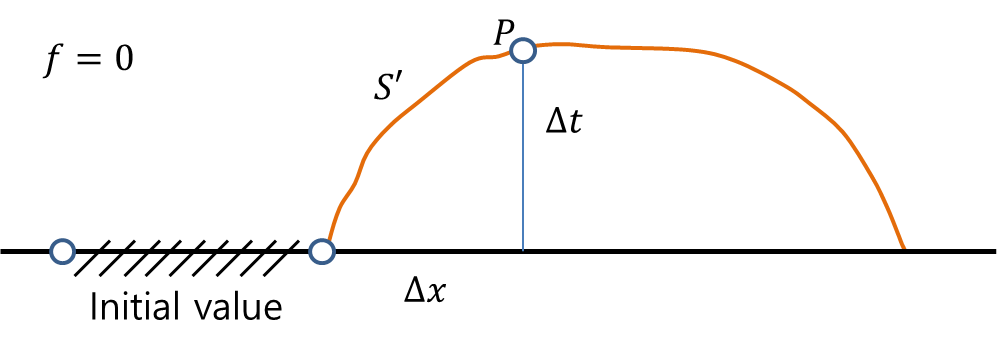
\includegraphics[scale=0.6]{11}
\end{center}
\end{figure}
If $\frac{\Delta t}{\Delta x} < \mu^{-1/2}$, can find $S'$ with $|D\tau |< \mu^{-1/2}$ such that $P\in D$ and $S_0$ outside support of data so $\sum_{i,j} a^{ij} \tau_{x_i} \tau_{x_j} \leq \mu |D\tau|^2 <1$. Thus $u=0$ at $P$. i.e.
\begin{align*}
\frac{\Delta t}{\Delta x} < \mu^{-1/2} \quad \text{implies we must tarvel faster than } \mu^{1/2} \text{ to travel from supp(Data) to } P
\end{align*}
\s

Using this property, we can construct solutions on \emph{unbounded domains} by reducing locally to a bounded problem and using this uniqueness result.
\begin{itemize}
\item Find $D$ containing $P$ with $S'$ space-like 
\item Put an artificial boundary outside $D$.
\item Use uniqueness to see that inside $D$, solving on the whole domain gives the same answer as solving on the bounded region.
\end{itemize}
\begin{figure}[h]
	\begin{center}
		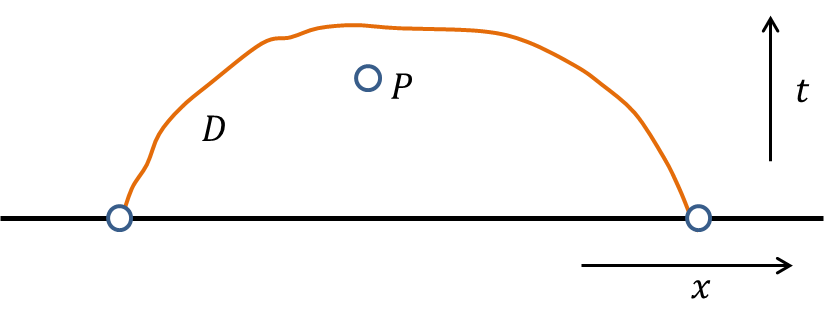
\includegraphics[scale=0.6]{13}
	\end{center}
\end{figure}
\end{document}